\begin{figure}
	\begin{subfigure}{.45\textwidth}
		\centering\begin{tikzpicture}
			\tikzmath{
						\length=4;	\height=3;
			}
			\draw (0,0) rectangle (\length,\height) node [midway] {$\mathscr{M}_{i,j}=1$};
			\node [above] at (0,\height+.1) {1};
			\node [above] at (\length/2,\height+.1) {j};
			\node [above] at (\length,\height+.1) {n};
			\path (0,\height+.1) -- (\length/2,\height+.1) node [above,midway] {$\cdots$} -- (\length,\height+.1) node [above,midway] {$\cdots$};

			\node [left] at (-.1,\height-.1) {1};
			\node [left] at (-.1,\height/2) {i};
			\node [left] at (-.1,0) {n};
			\path (-.1,\height-.1) -- (-.1,\height/2) node [left,midway] {$\vdots$} -- (-.1,0) node [left,midway] {$\vdots$};
		\end{tikzpicture}
		\caption[Matrix of children]{Matrix of children $\mathscr{M}_{i,j}=1$ if j is children of i and 0 otherwise.}\label{fig:mat}
	\end{subfigure}
	\begin{subfigure}{.45\textwidth}
		\centering\begin{tikzpicture}[implies/.style={double,double equal sign distance,-implies}]
			\tikzmath{
						\length=1;	\height=3;
						%\length2=5-1.25;	\height2=1;
			}
			\draw (0,0) rectangle (\length,\height) node [midway] {$V^s$[i]};
			\node [above] at (\length/2,\height+.1) {1};
			\node [left] at (-.1,\height-.1) {1};
			\node [left] at (-.1,\height/2) {i};
			\node [left] at (-.1,0) {n};
			\path (-.1,\height-.1) -- (-.1,\height/2) node [left,midway] {$\vdots$} -- (-.1,0) node [left,midway] {$\vdots$};

			\draw (\length+.25,\height/2) edge[implies] (\length+1,\height/2);

			\node [above] at (\length+1.25,2.1) {1};
			\node [above] at (\length+1.25+3.75/2,2.1) {j};
			\node [above] at (\length+1.25+3.75,2.1) {n};
			\path (\length+1.25,2.1) -- (\length+1.25+3.75/2,2.1) node [above,midway] {$\cdots$} -- (\length+1.25+3.75,2.1) node [above,midway] {$\cdots$};
			\draw (\length+1.25,\height/2-.5) rectangle (\length+5,\height/2+.5) node [midway] {$V^c_i$[j]};
		\end{tikzpicture}
		\caption{Vector of seeds and reconstructed vector of children}\label{fig:vect}
	\end{subfigure}\\
	\begin{subfigure}{.45\textwidth}
		\centering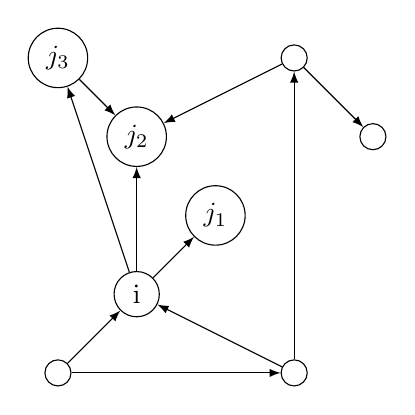
\begin{tikzpicture}
			\node [draw,circle] (N0) at (0,0) {};
			\node [draw,circle] (N1) at (1,1) {i};
			\node [draw,circle] (N2) at (2,2) {$j_1$};
			\node [draw,circle] (N3) at (3,0) {};
			\node [draw,circle] (N4) at (1,3) {$j_2$};
			\node [draw,circle] (N5) at (0,4) {$j_3$};
			\node [draw,circle] (N6) at (3,4) {};
			\node [draw,circle] (N7) at (4,3) {};
			
			\draw [-latex] (N0) -- (N1);
			\draw [-latex] (N1) -- (N2);
			\draw [-latex] (N1) -- (N4);
			\draw [-latex] (N1) -- (N5);
			\draw [-latex] (N5) -- (N4);
			\draw [-latex] (N6) -- (N4);
			\draw [-latex] (N3) -- (N1);
			\draw [-latex] (N0) -- (N3);
			\draw [-latex] (N3) -- (N6);
			\draw [-latex] (N6) -- (N7);
		\end{tikzpicture}
		\caption{Full network}\label{fig:net}
	\end{subfigure}
	\begin{subfigure}{.45\textwidth}
		\centering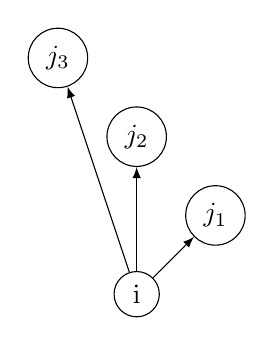
\begin{tikzpicture}
			%\node [draw,circle] (N0) at (0,0) {N0};
			\node [draw,circle] (N1) at (1,1) {i};
			\node [draw,circle] (N2) at (2,2) {$j_1$};
			%\node [draw,circle] (N3) at (3,0) {N3};
			\node [draw,circle] (N4) at (1,3) {$j_2$};
			\node [draw,circle] (N5) at (0,4) {$j_3$};
			%\node [draw,circle,color=gray!50] (N6) at (3,4) {N6};
			%\node [draw,circle,color=gray!50] (N7) at (4,3) {N7};
			
			%\draw [-latex] (N0) -- (N1);
			\draw [-latex] (N1) -- (N2);
			\draw [-latex] (N1) -- (N4);
			\draw [-latex] (N1) -- (N5);
			%\draw [-latex] (N5) -- (N4);
			%\draw [-latex] (N6) -- (N4);
			%\draw [-latex] (N3) -- (N1);
			%\draw [-latex] (N0) -- (N3);
			%\draw [-latex] (N3) -- (N6);
			%\draw [-latex] (N6) -- (N7);
		\end{tikzpicture}
		\caption{Only child of neuron i}\label{alg:vect}
	\end{subfigure}
	\caption{Algorithm for generating erdos-reynii graph in memory (a and c) and reconstructible (b and d)}
	\label{fig:rec}
\end{figure}
